First of all, let us examine the different ways by which
antibodies are naturally used by the immune system to combat
a pathogen infection. There are four of them, complementary of each other.

The key point here is that the antibodies allow for a specific recognition
of an antigen, and allow the immune system to act on it after it has
been detected. The antibodies on their own do not kill nor suppress any pathogen,
but act as the "recognition" part of the whole immune system.

\subsubsection{Antigen neutralization}

\begin{figure}[H]
    \begin{minipage}{0.55\textwidth}
        The most simple way antibodies can act against a pathogen is by
        \emph{neutralization} : the antibodies specific to an epitope of the
        antigen bind to this epitope and form together a complex that surround
        the pathogen \cite{langermans_antimicrobial_1994}.
        It is thus geometrically prevented to act as it normally would 
        by infecting the nearby cells.

        Antibodies acting in this manner are called \emph{neutralizing antibodies}
        or NAbs. The neutralized pathogen cannot approach the cell and
        bind to its surface receptors, thus making it ineffective. 
        The resulting complex can then be eliminated.
    \end{minipage}\hfill
    \begin{minipage}{0.35\textwidth}
        \centering
        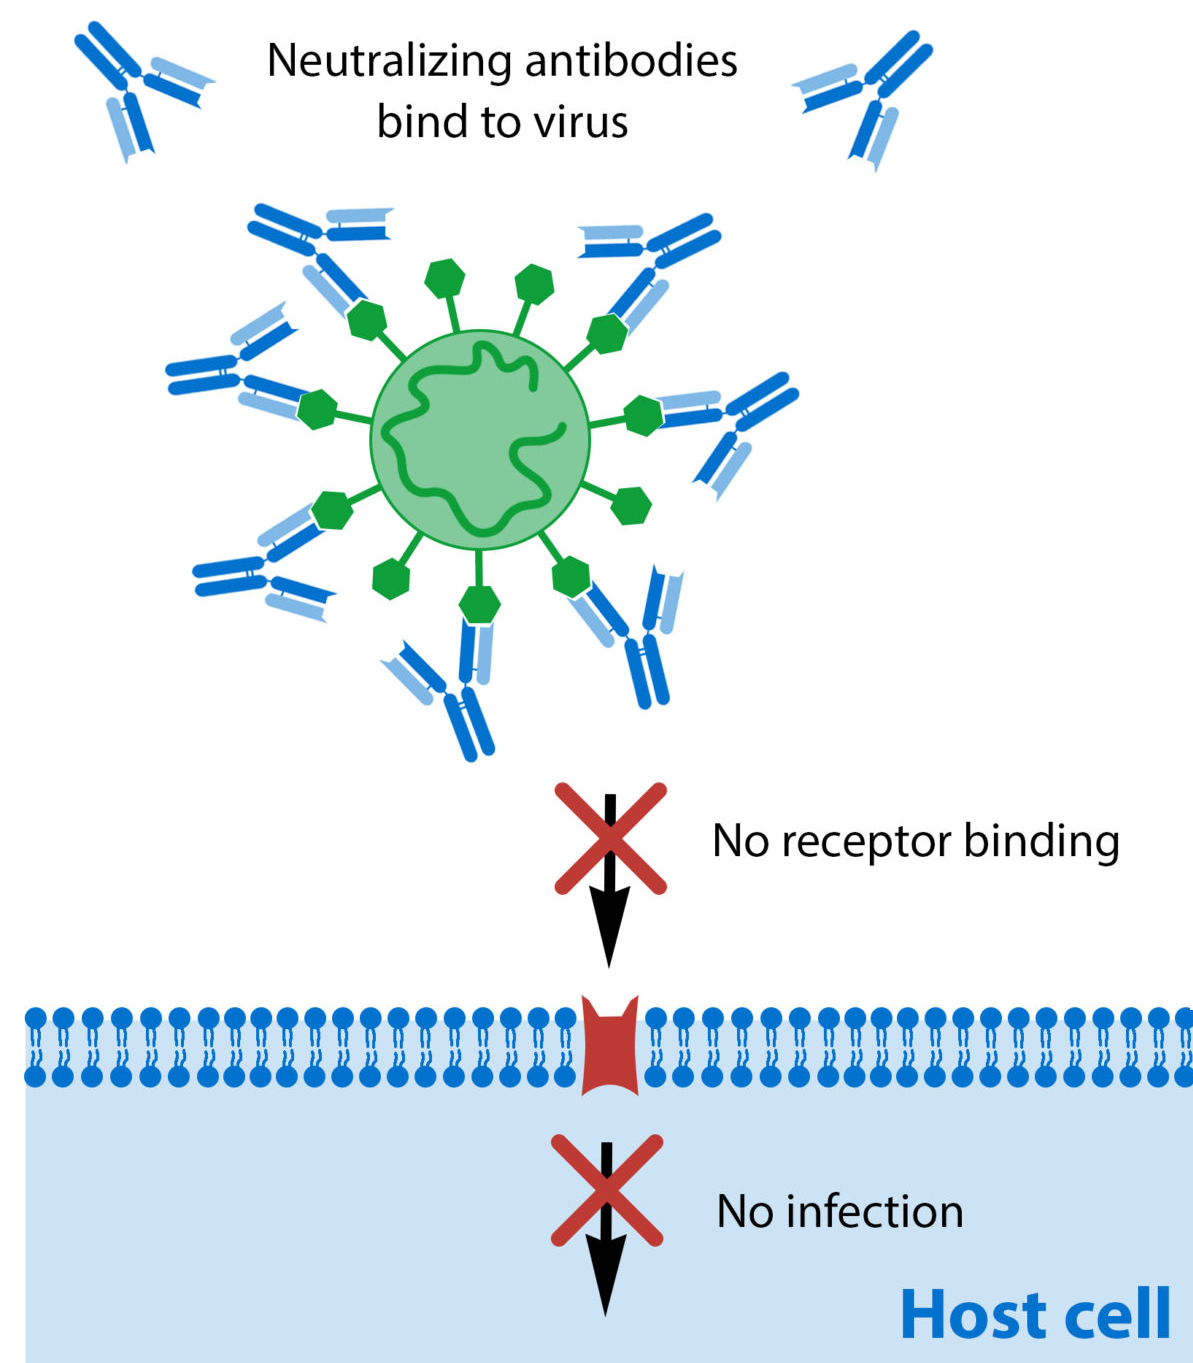
\includegraphics[width=\textwidth]{../Images/neutralization.png}   
        \caption{Neutralization of a pathogen by antibodies}
        \label{fig:neutralization}
    \end{minipage}
\end{figure}


\subsubsection{Antibody-Dependent Cellular Phagocytosis (ADCP)}

Another way by which antibodies help acting against a pathogen is very
close to neutralization. Indeed, once an antigen-antibody complex has been
created, some Fc receptor expressive immune effector cells can come into action
and act on the pathogen. 

Some cells, such as \emph{macrophage} cells but also natural killer or B lymphocytes, 
can bind to the Fc domain
of immunoglobulins attached to pathogens or infected -- or tumor -- cells
using their Fc receptors, which are trans membrane proteins \cite{fridman_fc_1991}. 
The phagocytic or cytotoxic activity of the cell is then activated \cite{tay_antibody-dependent_2019}.
This mechanism allow for the precise elimination of antigenic material, the antibodies
permitting specific detection of the pathogen or undesirable cell, and the effector cells
killing and eliminating the antigen.

\subsubsection{Antibody-Dependent Cell Cytotoxicity (ADCC)}

\subsubsection{Complement-Dependent Cell Cytotoxicity (CDCC)}
